%!TEX program = xelatex
\documentclass[a4paper,12pt]{report}
\usepackage{ctex}
%\usepackage{xeCJK}
\usepackage{times}
\usepackage{graphicx,float}
\usepackage{setspace}
\usepackage{fancyhdr}
% \usepackage{graphicx}
\usepackage{wrapfig}
\usepackage{array}
\usepackage{fontspec,xunicode,xltxtra}
\usepackage{titlesec}
\usepackage{titletoc}
\usepackage[titletoc]{appendix}
\usepackage[top=30mm,bottom=30mm,left=20mm,right=20mm]{geometry}
\usepackage{cite}
\usepackage{listings}
\usepackage[framed,numbered,autolinebreaks,useliterate]{mcode} % 插入代码
\XeTeXlinebreaklocale "zh"
\XeTeXlinebreakskip = 0pt plus 1pt minus 0.1pt

%---------------------------------------------------------------------
%	页眉页脚设置
%---------------------------------------------------------------------
\fancypagestyle{plain}{
	\pagestyle{fancy}      %改变章节首页页眉
}

\pagestyle{fancy}
\lhead{\kaishu~``科研素质训练''课程报告~}
\rhead{\kaishu~~张三~~}
\cfoot{\thepage}

%---------------------------------------------------------------------
%	章节标题设置
%---------------------------------------------------------------------
%\titleformat{\section}{\centering\zihao{-1}\heiti}{报告\chinese{section}}{1em}{}
%\titlespacing{\section}{0pt}{*0}{*6}

%---------------------------------------------------------------------
%	摘要标题设置
%---------------------------------------------------------------------
\renewcommand{\contentsname}{\centerline{\zihao{2} 目\quad 录}}

%---------------------------------------------------------------------
%	参考文献设置
%---------------------------------------------------------------------
\renewcommand{\bibname}{\centerline{\zihao{2}{参\hspace{0.5em}考\hspace{0.5em}文\hspace{0.5em}献}}}

%---------------------------------------------------------------------
%	引用文献设置为上标
%---------------------------------------------------------------------
\makeatletter
\def\@cite#1#2{\textsuperscript{[{#1\if@tempswa , #2\fi}]}}
\makeatother

%---------------------------------------------------------------------
%	目录页设置
%---------------------------------------------------------------------
%\titlecontents{chapter}[0em]{\songti\zihao{-4}}{\thecontentslabel\ }{}
%{\hspace{.5em}\titlerule*[4pt]{$\cdot$}\contentspage}
%\titlecontents{section}[2em]{\vspace{0.1\baselineskip}\songti\zihao{-4}}{\thecontentslabel\ }{}
%{\hspace{.5em}\titlerule*[4pt]{$\cdot$}\contentspage}
%\titlecontents{subsection}[4em]{\vspace{0.1\baselineskip}\songti\zihao{-4}}{\thecontentslabel\ }{}
%{\hspace{.5em}\titlerule*[4pt]{$\cdot$}\contentspage}
\renewcommand\thesection{\arabic{section}}
\renewcommand\thesubsection{\arabic{section}.\arabic{subsection}}

\begin{document}


%---------------------------------------------------------------------
%	封面设置
%---------------------------------------------------------------------
\begin{titlepage}
	\begin{center}
		
    
\includegraphics[width=1.0\textwidth]{figure//nankai.jpg}\\
    % \vspace{10mm}
    % \textbf{\zihao{2}\kaishu{软件学院}}\\[0.8cm]
    \vspace{50mm}
    \textbf{\zihao{1}\heiti{ 《科研素质训练》课程报告}}\\[3cm]
    \textbf{\zihao{2}\heiti{ 报告题目}}\\[3cm]
	\vspace{\fill}
	
\setlength{\extrarowheight}{3mm}
{\songti\zihao{3}	
\begin{tabular}{rl}
	
	{\makebox[4\ccwd][s]{学\qquad 院:}}& ~\kaishu 软件学院\\
	
	{\makebox[4\ccwd][s]{姓\qquad 名:}}& ~\kaishu 张三~~ \\

    {\makebox[4\ccwd][s]{学\qquad 号:}}& ~\kaishu 001~~ \\


\end{tabular}
 }\\[2cm]
\vspace{\fill}
\zihao{4}
2021\textasciitilde 2022第一学期\\
使用\LaTeX 撰写于\today
	\end{center}	
\end{titlepage}


%---------------------------------------------------------------------
%  目录页
%---------------------------------------------------------------------
\tableofcontents % 生成目录

%---------------------------------------------------------------------
%
%---------------------------------------------------------------------
\newpage
\section{第一节标题}
\setcounter{page}{1}
\begin{spacing}{1.5}
\songti\zihao{-4}
通过本课程学习...
\subsection{小节标题}
\subsection{小节标题}

\end{spacing}
\section{第二节标题}
\begin{spacing}{1.5}
\subsection{小节标题}
\begin{itemize}
  \item 要点一 \cite{GDLIII}
  \item 要点二 \cite{einstein}
  \item 要点三 \cite{knuthwebsite}
\end{itemize}

\subsection{小节标题}

\end{spacing}

\section{结语}
\zihao{-4}\songti
\begin{spacing}{1.5}
软件截图如图~\ref{pic1}所示。
\begin{figure}[!ht]
  \centering
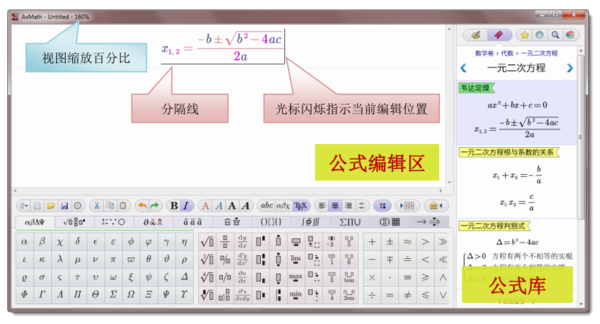
\includegraphics[width=12cm]{figure/calculator.png}\caption{计算器截图}\label{pic1}
\end{figure}

\end{spacing}





%---------------------------------------------------------------------
%  %参考文献设置
%---------------------------------------------------------------------
 \addcontentsline{toc}{section}{参考文献}

\bibliographystyle{abbrv}
\bibliography{bibliography}
%\begin{thebibliography}{1}
%
%\bibitem{einstein}
%A.~Einstein.
%\newblock {Zur Elektrodynamik bewegter K{\"o}rper}.
%\newblock {\em Annalen der Physik}, 322(10):891--921, 1905.
%
%\bibitem{knuthwebsite}
%D.~Knuth.
%\newblock Knuth: Computers and typesetting.
%
%\bibitem{GDLIII}
%M.~Thielscher.
%\newblock {GDL-III}: A description language for epistemic general game playing.
%\newblock In {\em Proceedings of the 26th International Joint Conference on
%  Artificial Intelligence ({IJCAI'17})}, pages 1276--1282, 2017.
%
%\end{thebibliography}
 %\begin{thebibliography}{99}
% \songti \zihao{-4} 	
% 	\bibitem{Leslie.{1994}}
% 	Leslie Lamport. LATEX: A Document Preparation System.AddisonWesley, Reading, Massachusetts, second edition, 1994, ISBN 0-201-52983-1.
%	
% 	\bibitem{Donald.{1984}}
% 	Donald E. Knuth. The TEXbook, Volume A of Computers and Typesetting,Addison Wesley, Reading, Massachusetts, second edition, 1984,ISBN 0-201-13448-9.
%
%	
% \end{thebibliography}

%---------------------------------------------------------------------
%  附录设置
%---------------------------------------------------------------------
% \titleformat{\section}{\heiti\Large}{附录~\Alph{section}}{11pt}{\Large}
% \titlespacing{\chapter}{0pt}{*-4}{*4}
%
% \lstset{breaklines}                %自动将长的代码行换行排版
% \lstset{extendedchars=false}
% \lstset{language=Matlab}
% \renewcommand{\thechapter}{附录\Alph{section}.}
% \appendix
% \begin{appendix}
	
	

 %\end{appendix}
		

\end{document}
